\documentclass[letterpaper]{article}
\usepackage{amsmath,amsfonts}
\usepackage[margin=.75in]{geometry}
\usepackage[]{graphicx}
\usepackage{listings}
\usepackage{color}
\usepackage{textcomp}
\definecolor{listinggray}{gray}{0.9}
\definecolor{lbcolor}{rgb}{0.9,0.9,0.9}
\lstset{
	backgroundcolor=\color{lbcolor},
	tabsize=4,
	rulecolor=,
	language=Python,
        basicstyle=\scriptsize,
        upquote=true,
        aboveskip={1.5\baselineskip},
        columns=fixed,
        showstringspaces=false,
        extendedchars=true,
        breaklines=true,
        prebreak = \raisebox{0ex}[0ex][0ex]{\ensuremath{\hookleftarrow}},
        frame=single,
        showtabs=false,
        showspaces=false,
        showstringspaces=false,
        identifierstyle=\ttfamily,
        keywordstyle=\color[rgb]{0,0,1},
        commentstyle=\color[rgb]{0.133,0.545,0.133},
        stringstyle=\color[rgb]{0.627,0.126,0.941},
}
\addtolength{\parskip}{\baselineskip}

\title{Statistical Mechanics: HW 6}
\author{Truman Ellis}

\begin{document}
\maketitle
Our goal is to use umbrella sampling and Metropolis Monte Carlo to estimate the
ratio $P(q_{\text{lowest minimum}})/P(q_{\text{barrier}})$ for the Muller
potential. We do this by tracing out the path shown in red in Figure
\ref{fig:path}. At each point along the path, we define a biasing potential 
\[
V(x,y) = k([(x,y)-q_i]\cdot e_{q_i})^2
\]
where $q_i$ is the sample point, $e_{q_i}$ is the tangent to the sample curve at
that point, and $k$ is the strength of the biasing potential. Then we run a
small Metropolis Monte Carlo simulation starting at $q_i$ with the Muller plus
biasing potential. Within the MMC simulation, we chose a maximum window size of
$10^{-2}\times10^{-2}$. This produced reasonable acceptance rates. We chose a
biasing strength of 5000, which effectively channeled each simulation, but
allowed enough overlap between simulations to glue all of the simulations
together. After each mini simulation, I had an array of positions that the
particle had visited. I then calculated the signed distance away from the 
reaction coordinate for each data point. With 2000 steps per simulation, 
this data fell into a nice Gaussian distribution (for high enough $k$). My first
approach was to compute a histogram of this data then take the log and add
$\beta V$. The challenge with this approach was finding an adequate way of
gluing together the data from each of the mini simulations. After some further
thought, I decided to make use of the fact that the data followed such a nice
Gaussian distribution. I instead fit the data to a normal distribution via its
mean and standard deviation. Taking the log of this and adding $\beta V$ gave me
a function that I could evaluate anywhere along the line. By evaluating two
successive functions at the half nodes, I could calculate a shifting constant
and vertically shift the second function in order to match the values. 

I ran several simulations at varying sample densities, but 3200 sample points
appeared to produce plots that lined up nicely, as shown in Figures
\ref{fig:path} and \ref{fig:logP}. By subtracting the minimum value from the
maximum, we get 
\[
\log(P(q_{\text{lowest minimum}}))-\log(P(q_{\text{barrier}}))
=\log\left( P(q_{\text{lowest minimum}})/P(q_{\text{barrier}}) \right)\,.
\]
Then if we raise $e$ to this value, we get the desired ratio of probabilities.
For the simulation shown below, I got 
\[
\log( P(q_{\text{lowest minimum}})/P(q_{\text{barrier}})) = 578.42
\]
or 
\[
P(q_{\text{lowest minimum}})/P(q_{\text{barrier}}) = e^{578.41}\approx 1.6e+251\,.
\]

\begin{figure}[h]
\begin{center}
\includegraphics[width=7.5in]{path3200.pdf}
\end{center}
\caption{Sample path for umbrella sampling with mini Metropolis Monte Carlo
simulations at each point}
\label{fig:path}
\end{figure}

\begin{figure}[h]
\begin{center}
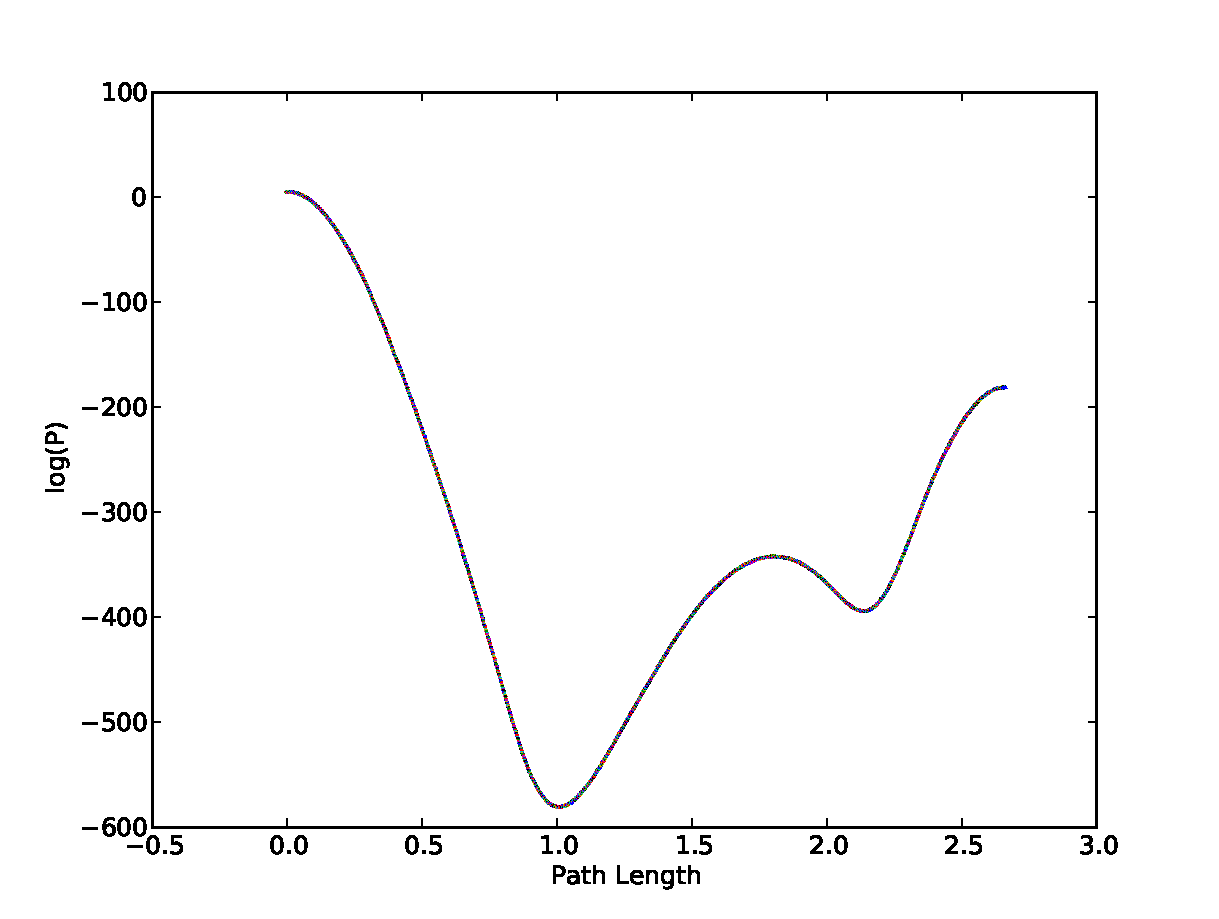
\includegraphics[width=7.5in]{logP3200.pdf}
\end{center}
\caption{Log of the probability evaluated along the sample path}
\label{fig:logP}
\end{figure}

\newpage 
\clearpage
\lstinputlisting[language=Python,title={HW6.py}]{HW6.py}
\end{document}
